\documentclass{uimppracticas}

%%%%%%%%%%%%%%%%%%%%%%%%%%%%%%%%%%%%%%%%%%%%%%%%%%%%%%%%%%%%%%%%%%%%%%%%%%%%%%%%
%%%                   Plantilla Prácticas UIMP                               %%%
%%%                Universidad Internacional Menéndez Pelayo                 %%%
%%%                   Laura Rodríguez Navas                                  %%%
%%%%%%%%%%%%%%%%%%%%%%%%%%%%%%%%%%%%%%%%%%%%%%%%%%%%%%%%%%%%%%%%%%%%%%%%%%%%%%%%

%Permitir cabeceras y pie de páginas personalizados
\pagestyle{fancy}

%Path por defecto de las imágenes
\graphicspath{ {./images/} }

%Declarar formato de encabezado y pie de página de las páginas del documento
\fancypagestyle{doc}{
	%Cabecera
	\headerpr[1]{}{}{Datos temporales y complejos}
	%Pie de Página
	\footerpr{}{}{{\thepage} de \pageref{LastPage}}
}

%Declarar formato de encabezado y pie del título e indice
\fancypagestyle{titu}{%
	%Cabecera
	\headerpr{}{}{}
	%Pie de Página
	\footerpr{}{}{}
}


\appto\frontmatter{\pagestyle{titu}}
\appto\mainmatter{\pagestyle{doc}}

%"mystyle" code listing set
\lstset{style=mystyle}
\renewcommand{\lstlistingname}{Algoritmo}% Listing -> Algoritmo
\renewcommand{\lstlistlistingname}{Lista de \lstlistingname s}% List of Listings -> List of Algoritmos

\begin{document}
	
%Comienzo formato título
\frontmatter

%Portada (Centrado todo)
\centeredtitle{./images/LogoUIMP.png}{Máster Universitario en Investigación en Inteligencia Artificial}{Curso 2020-2021}{Datos temporales y complejos}{Evaluación Data Streams: Metodologías}

\begin{center}
	\large Noviembre 2020
\end{center}

\vspace{30mm}

\begin{flushright}
	{\bf Laura Rodríguez Navas}\\
	\textbf{DNI:} 43630508-Z\\
	\textbf{e-mail:} \href{rodrigueznavas@posgrado.uimp.es}{rodrigueznavas@posgrado.uimp.es}
\end{flushright}

\newpage

%Índice
\tableofcontents

\newpage

%Comienzo formato documento general
\mainmatter

\section{Ejercicio 1}

Sea un fichero de texto que contiene una secuencia desordenada de valores enteros del 1 al N, pero al que le falta uno de los valores. Escriba un programa en cualquier lenguaje de programación tal que lea un fichero como el anterior y dé en el menor tiempo posible y con el menor uso de memoria respuesta a cuál es el número que falta en la secuencia. Pruébelo para N suficientemente grande. Haga una tabla con el tiempo de computación necesario y la memoria usada para al menos 10 ejecuciones con distintos valores de N.

\lstinputlisting[language=Python, caption=Búsqueda del número que falta en la secuencia.]{code/exercise_one/find_number.py}

A continuación, podemos ver la tabla con el tiempo de computación (tCompu) necesario y la memoria usada (uMem) de 10 ejecuciones con distintos valores de N. El tiempo de computación se obtiene en segundos y la memoria usada en MB. 

\begin{center}
	\begin{tabular}{ |c|c|c|c|c| } 
		\hline
		id & N & tCompu & uMem \\
		\hline
		1 &  100 &      0.0010001659 &    0.0234375 \\ 
		2 &  1000 &     0.0030002594 &    0.0546875 \\
		3 &  10000 &    0.0190010071 &    0.74609375 \\ 
		4 &  50000 &    0.1000056267 &    1.46875 \\ 
		5 &  100000 &   0.2060117722 &    3.11328125 \\ 
		6 &  500000 &   1.1400651932 &    9.69921875 \\ 
		7 &  1000000 &  2.2931311131 &   19.5625 \\ 
		8 &  5000000 &  12.1846969128 &  97.375 \\ 
		9 &  10000000 & 24.5054016113 & 193.1328125 \\ 
		10 & 15000000 & 37.9671714306 & 289.20703125 \\ 
		\hline
	\end{tabular}
\end{center}

Se puede observar que cuanto mayor sea el data stream, mayor tiempo de computación y mayor memoria se usará durante la ejecución del programa.

Nota: Genere los datos del fichero de entrada con otro programa que lo escriba, esto es dado dos enteros x y N (x entre 1 y N) construya un programa que escriba en un fichero los números del 1 al N excepto x de manera desordenada.

\lstinputlisting[language=Python, caption=Generador de los datos del fichero de entrada.]{code/exercise_one/generate_data.py}

\section{Ejercicio 2}

Sea una secuencia desordenada de N números (N suficientemente grande). Queremos encontrar mediante muestreo un número en ella que sea mayor que el tercer cuartil, esto es, que esté en el 25\% superior de los valores de la secuencia. Para ello una posibilidad es escoger aleatoriamente k valores y quedarnos con el mayor de esos k. ¿Cuál es el menor k posible para que el error sea menor que 0.3? Es decir, que en media de cada 10 veces que repitamos el experimento nos equivoquemos en menos de 3. ¿Y si queremos que la tasa de error baje al 0.1, cuánto debe valer k? 

El menor k posible para que el error sea menor que 0.3:

\begin{center}
	$ k = \log_2(1/0.3) \approx 2 $
\end{center}

El menor k posible para que el error sea menor que 0.1:

\begin{center}
	$ k = \log_2(1/0.1) \approx 4 $
\end{center}

Haga un programa similar al mostrado en el vídeo que demuestre experimentalmente los valores de k calculados de forma teórica.

\lstinputlisting[language=Python, caption=Demostración experimental de los valores de k calculados de manera teórica.]{code/exercise_two/cota_del_error.py}

\newpage

Con k = 2, el resultado obtenido de la ejecución del algoritmo anterior es 0.236167, y de esta manera se demuestra que la probabilidad del error es menor a 0.3.

Con k = 4, el resultado obtenido de la ejecución del algoritmo anterior es 0.043217 y se demuestra que la probabilidad del error es menor a 0.1.

\section{Ejercicio 3}

Supongamos tenemos una secuencia de valores con la frecuencia que se indica:

Valor: 1 Frecuencia: 7\\
Valor: 2 Frecuencia: 3\\
Valor: 3 Frecuencia: 4\\
Valor: 4 Frecuencia: 5\\
Valor: 5 Frecuencia: 9\\
Valor: 6 Frecuencia: 10\\
Valor: 7 Frecuencia: 8\\
Valor: 8 Frecuencia: 1\\
Valor: 9 Frecuencia: 9\\
Valor: 10 Frecuencia: 4\\

Si agrupamos en un histograma de 6 intervalos o bloques de igual frecuencia la salida sería:

\begin{center}
	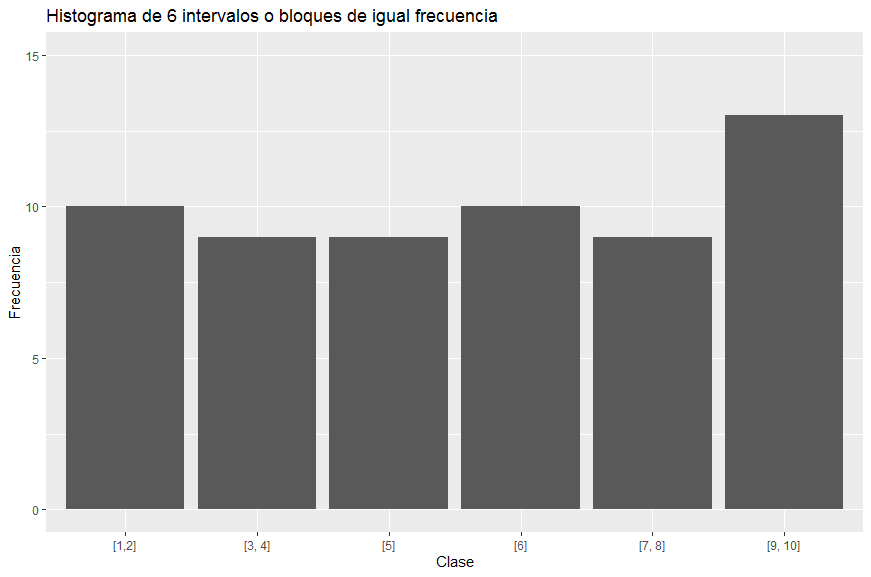
\includegraphics[scale=0.7]{code/exercise_three/hist_1}
\end{center}

Si agrupamos en un histograma de 4 intervalos o bloques de igual frecuencia la salida sería:

\begin{center}
	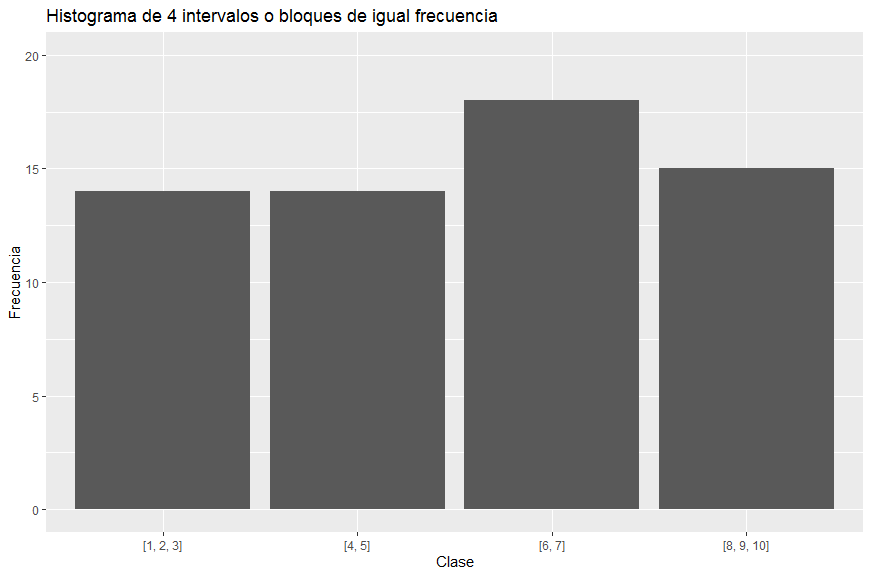
\includegraphics[scale=0.6]{code/exercise_three/hist_2}
\end{center}

Si agrupamos en un histograma de 6 intervalos o bloques minimizando la varianza sería:

\begin{center}
	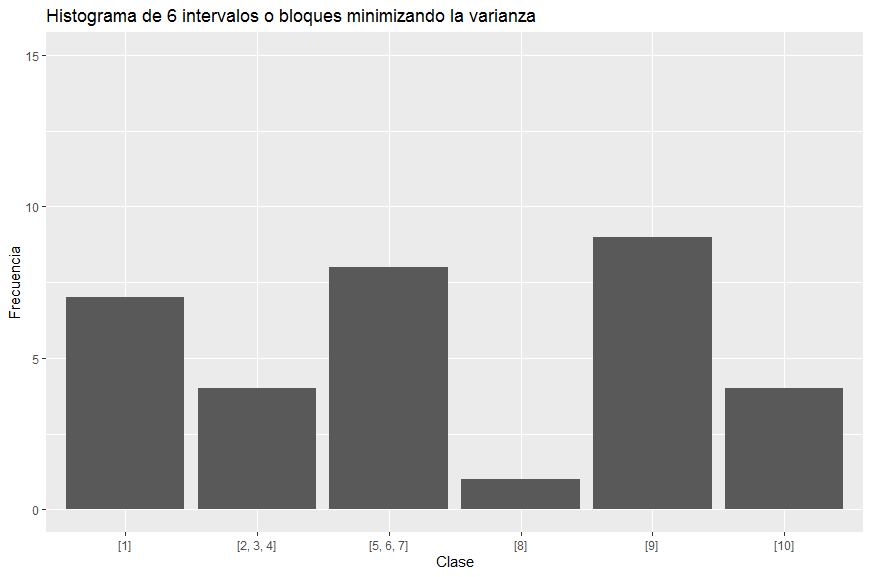
\includegraphics[scale=0.7]{code/exercise_three/hist_3}
\end{center}

\section{Ejercicio 4}

Calcula en el ejemplo de Count-Min Sketch que se puede ver en el vídeo los conjuntos sobre los que habría que hallar el mínimo para calcular la frecuencia de D, E y F. 

Dado el data stream:

\begin{center}
	(A, 1), (B, 2), (C, 5), (B, 4), (E, 8), (D, 7), (C, 8), (F, 5), (G, 10), (C, 5), (H, 3)
\end{center}

Dada la tabla:

\begin{center}
	\begin{tabular}{|c|c|c|c|c|c|c|c|c|}
		\hline
		h$_{1}$(A)=5 & h$_{1}$(B)=1 & h$_{1}$(C)=2 & h$_{1}$(D)=1 & h$_{1}$(E)=2 & h$_{1}$(F)=6 & h$_{1}$(G)=2 & h$_{1}$(H)=3 & ... \\ \hline
		h$_{2}$(A)=6 & h$_{2}$(B)=3 & h$_{2}$(C)=4 & h$_{2}$(D)=3 & h$_{2}$(E)=4 & h$_{2}$(F)=1 & h$_{2}$(G)=5 & h$_{2}$(H)=4 & ... \\ \hline
		h$_{3}$(A)=1 & h$_{3}$(B)=4 & h$_{3}$(C)=5 & h$_{3}$(D)=2 & h$_{3}$(E)=6 & h$_{3}$(F)=3 & h$_{3}$(G)=3 & h$_{3}$(H)=6 & ... \\ \hline
	\end{tabular}
\end{center}

Obtenemos,

\begin{center}
	\begin{tabular}{|c|c|c|c|c|c|}
		\hline
		7+4+2 & 8+8+5+10 & +3 &  & +1 & +5 \\ \hline
		+5 &  & 7+4+2 & 3+8+8+5 & +10 & +1 \\ \hline
		+1 & +7 & 10+5 & 4+2 & 5+8+5 & 3+8 \\ \hline
	\end{tabular}
\end{center}

Donde el mínimo para calcular la frecuencia de A, B y C es:

\begin{itemize}
	\item \#(A) = min\{CM[1, h$_{1}$(A)], CM[2, h$_{2}$(A)], CM[3, h$_{3}$(A)\} = min\{1, 1, 1\} = 1 
	\item \#(B) = min\{CM[1, h$_{1}$(B)], CM[2, h$_{2}$(B)], CM[3, h$_{3}$(B)\} = min\{13, 13, 6\} = 6 
	\item \#(C) = min\{CM[1, h$_{1}$(C)], CM[2, h$_{2}$(C)], CM[3, h$_{3}$(C)\} = min\{31, 24, 18\} = 18
\end{itemize}

y el mínimo para calcular la frecuencia de D, E y F es:

\begin{itemize}
	\item \#(D) = min\{CM[1, h$_{1}$(D)], CM[2, h$_{2}$(D)], CM[3, h$_{3}$(D)\} = min\{13, 13, 7\} = 7 
	\item \#(E) = min\{CM[1, h$_{1}$(E)], CM[2, h$_{2}$(E)], CM[3, h$_{3}$(E)\} = min\{31, 24, 11\} = 11 
	\item \#(F) = min\{CM[1, h$_{1}$(F)], CM[2, h$_{2}$(F)], CM[3, h$_{3}$(D)\} = min\{5, 5, 15\} = 5
\end{itemize}

y el mínimo para calcular la frecuencia de G y H es:

\begin{itemize}
	\item \#(G) = min\{CM[1, h$_{1}$(G)], CM[2, h$_{2}$(G)], CM[3, h$_{3}$(G)\} = min\{31, 10, 15\} = 10 
	\item \#(H) = min\{CM[1, h$_{1}$(H)], CM[2, h$_{2}$(H)], CM[3, h$_{3}$(H)\} = min\{3, 24, 11\} = 3 
\end{itemize}

\newpage

¿En cuál se está cometiendo un error sobre el valor real?

En E. El valor mínimo para calcular la frecuencia de E es 11, mientras que el valor real de E es 8.

\addcontentsline{toc}{section}{Lista de Algoritmos}
\lstlistoflistings

Para esta actividad se han realizado una serie de desarrollos en Python y R que se pueden encontrar \href{https://github.com/lrodrin/masterAI/tree/master/A9/Data\%20Streams/methodologies}{\textbf{AQUÍ}}.

\end{document}
